\documentclass[12pt,a4paper]{article}
\usepackage[margin=2.5cm]{geometry}
\usepackage{fontspec}
\usepackage{graphicx}
\usepackage{float}
\usepackage{hyperref}
\usepackage{xcolor}
\usepackage{listings}
\usepackage{fancyhdr}
\usepackage{booktabs}

% All black/white - no colors
\hypersetup{
    colorlinks=true,
    linkcolor=black,
    urlcolor=blue
}

% Header/Footer
\pagestyle{fancy}
\fancyhf{}
\fancyhead[L]{\small ShoeShop - Kotlin Jetpack Compose}
\fancyhead[R]{\small \thepage}
\fancyfoot[C]{\small CS5450 Mobile Programming - Lakehead University}
\renewcommand{\headrulewidth}{0.4pt}

% Section formatting (black)
\makeatletter
\renewcommand\section{\@startsection{section}{1}{\z@}%
    {-3.5ex \@plus -1ex \@minus -.2ex}%
    {2.3ex \@plus.2ex}%
    {\Large\bfseries}}
\renewcommand\subsection{\@startsection{subsection}{2}{\z@}%
    {-3.25ex\@plus -1ex \@minus -.2ex}%
    {1.5ex \@plus .2ex}%
    {\large\bfseries}}
\makeatother

% Code listing style
\definecolor{codebg}{HTML}{F5F5F5}
\lstset{
    backgroundcolor=\color{codebg},
    basicstyle=\small\ttfamily,
    breaklines=true,
    frame=single,
    framerule=0.4pt,
    rulecolor=\color{black!30},
    xleftmargin=1em,
    framexleftmargin=1em,
    columns=fullflexible,
    keepspaces=true
}

\begin{document}

% ===== COVER PAGE =====
\begin{titlepage}
\centering
\vspace*{3cm}

{\Huge\bfseries ShoeShop}\\[0.5cm]
{\Large Kotlin Jetpack Compose Mobile Shopping App}

\vspace{2cm}

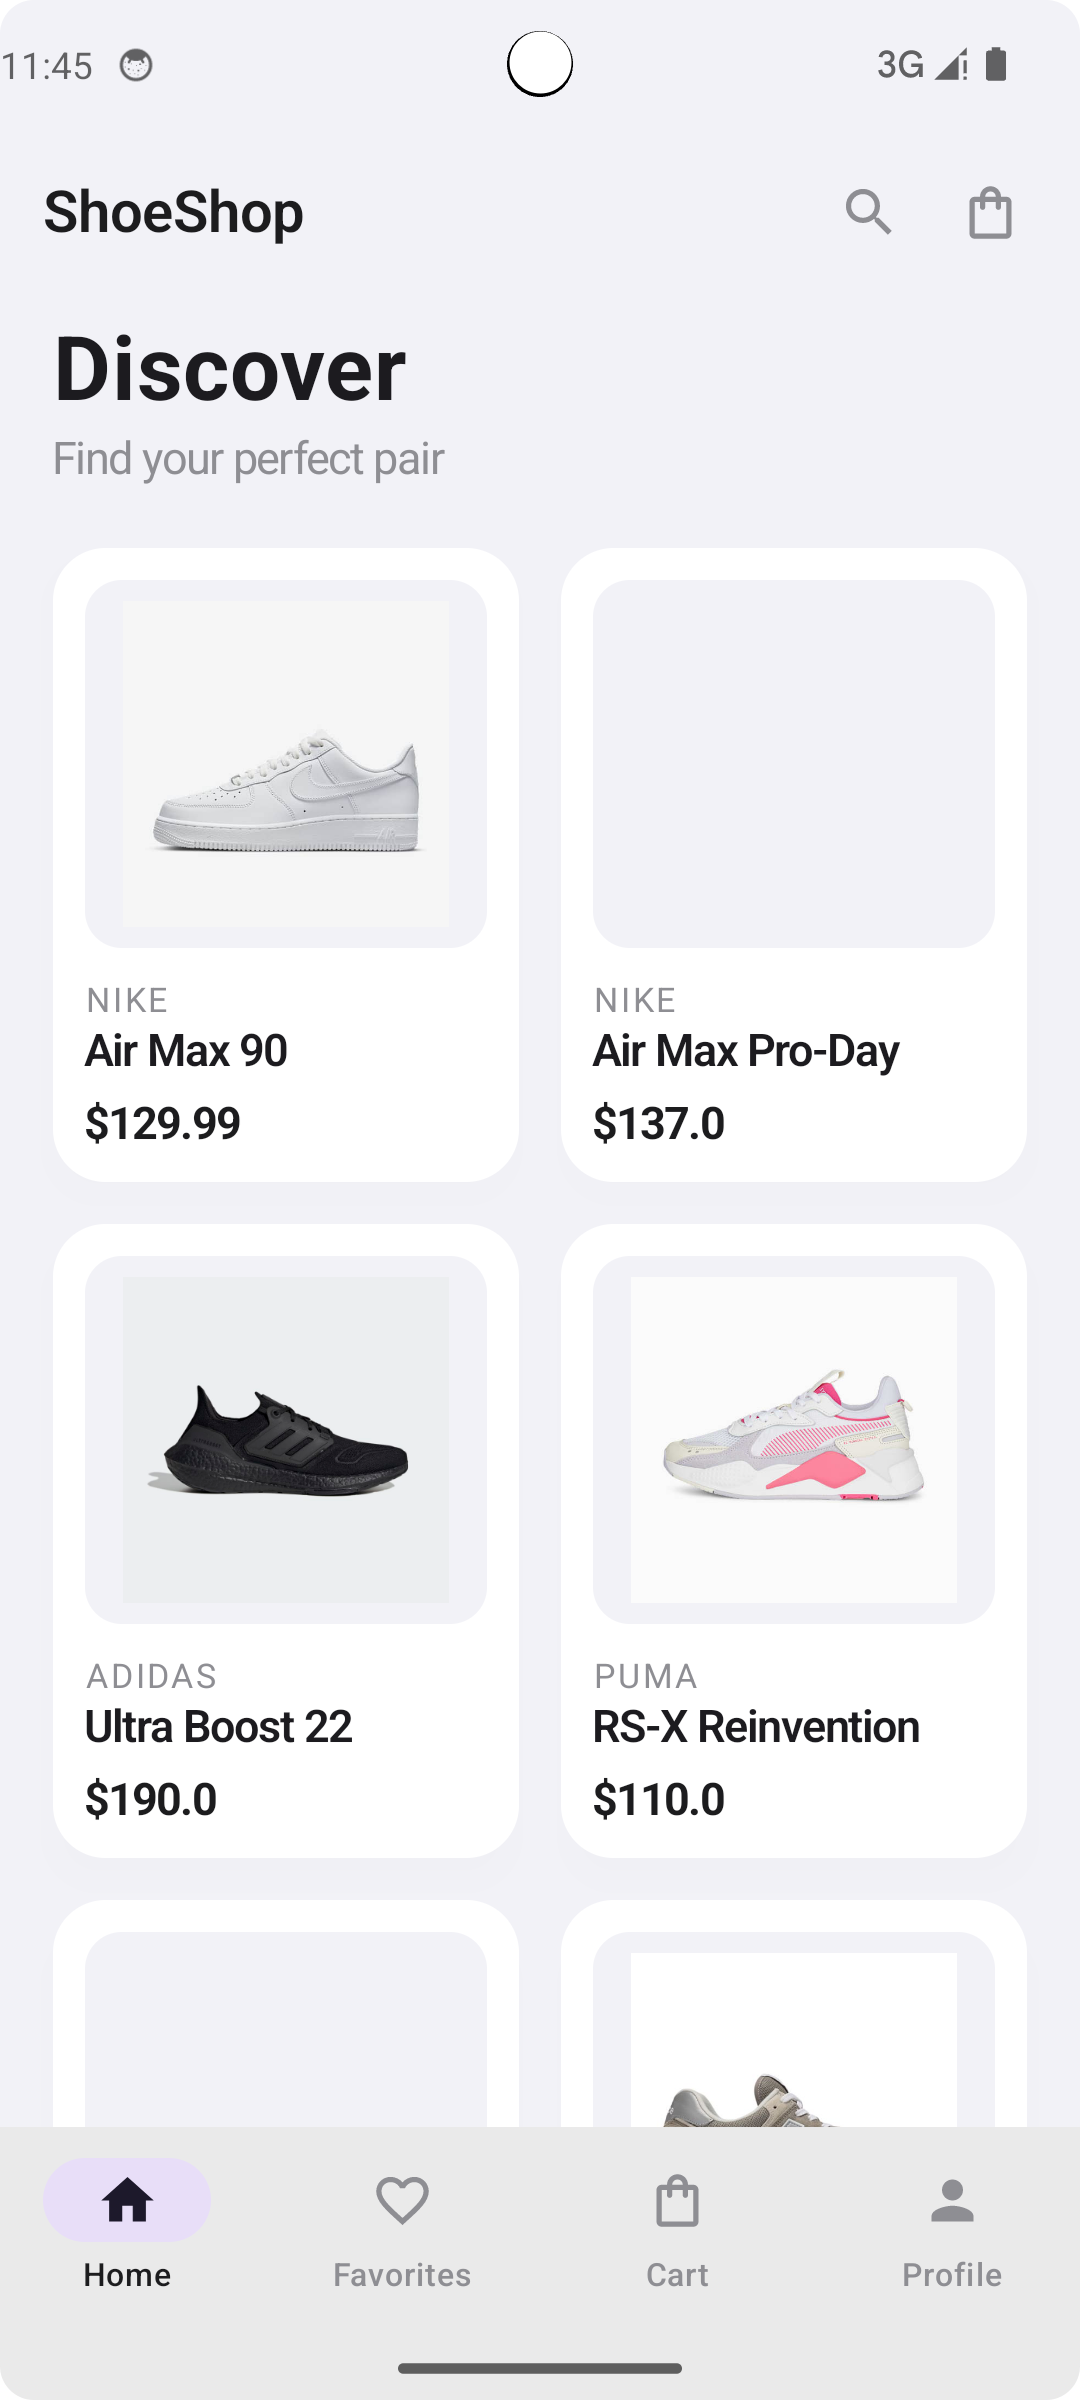
\includegraphics[width=0.35\textwidth]{Screenshots/Screenshot_20260504_234552.png}

\vspace{2cm}

{\large
\begin{tabular}{rl}
\textbf{Course:} & CS5450 Mobile Programming \\[0.3cm]
\textbf{Group:} & Group \#4 - Mobile Shop \\[0.3cm]
\textbf{Framework:} & Kotlin Jetpack Compose (Material3) \\[0.3cm]
\textbf{Platform:} & Android (API 26+) \\[0.3cm]
\textbf{Date:} & May 5, 2026 \\
\end{tabular}
}

\vfill
{\small Built with Android Studio | Kotlin 1.9.24 | Jetpack Compose | Material Design 3}
\end{titlepage}

% ===== TABLE OF CONTENTS =====
\tableofcontents
\newpage

% ===== SECTION 1: OVERVIEW =====
\section{Project Overview}

ShoeShop is a mobile shopping application built with \textbf{Kotlin Jetpack Compose} that demonstrates modern Android development (MAD) practices. The app allows users to:

\begin{itemize}
    \item Browse a catalog of shoes displayed in a responsive grid layout
    \item View detailed product information including description, price, and available sizes
    \item Add items to a shopping bag with quantity management
    \item View shopping bag total with itemized pricing
\end{itemize}

\subsection{Key Architecture Principles}
\begin{itemize}
    \item \textbf{ViewModel + StateFlow} --- Cart state managed in ViewModel, survives screen rotation
    \item \textbf{Type-Safe Navigation} --- Using @Serializable route objects (Gold Standard)
    \item \textbf{State Hoisting \& UDF} --- Stateless composables with unidirectional data flow
    \item \textbf{Material Design 3} --- Scaffold, TopAppBar, NavigationBar throughout
\end{itemize}

% ===== SECTION 2: GITHUB =====
\section{GitHub Public Repository}

\url{https://github.com/realzhengyuting-cloud/ShoeShop}

% ===== SECTION 3: SETUP =====
\section{How to Configure and Run}

\subsection{Prerequisites}
\begin{itemize}
    \item Android Studio Hedgehog (2023.1.1) or later
    \item JDK 17
    \item Android SDK 34
    \item Android Emulator or physical device (API 26+)
\end{itemize}

\subsection{Steps to Run}
\begin{enumerate}
    \item Clone the repository: \texttt{git clone https://github.com/realzhengyuting-cloud/ShoeShop.git}
    \item Open Android Studio
    \item Select \texttt{File > Open} and choose the \texttt{ShoeShop} folder
    \item Wait for Gradle sync to complete (first time may take a few minutes)
    \item Create a virtual device: \texttt{Tools > Device Manager > Create Virtual Device}
    \begin{itemize}
        \item Select \textbf{Pixel 6} (or any phone)
        \item Choose system image \textbf{API 34}
        \item Click Finish
    \end{itemize}
    \item Select the emulator from the device dropdown
    \item Click the \textbf{Run} button (green play icon) or press \texttt{Shift+F10}
\end{enumerate}

\subsection{Build Configuration}
\begin{table}[H]
\centering
\begin{tabular}{@{}ll@{}}
\toprule
\textbf{Component} & \textbf{Version} \\
\midrule
Kotlin Plugin & 1.9.24 \\
Compose Compiler & 1.5.14 \\
Navigation Compose & 2.8.5 \\
Lifecycle Runtime Compose & 2.7.0 \\
Serialization JSON & 1.6.3 \\
\bottomrule
\end{tabular}
\end{table}

% ===== SECTION 4: STRUCTURE =====
\section{Project Structure}

\begin{lstlisting}
ShoeShop/
|-- app/
|   |-- build.gradle.kts         (App-level build config)
|   +-- src/main/
|       |-- AndroidManifest.xml  (App manifest)
|       |-- java/com/example/shoeshop/
|       |   |-- MainActivity.kt         (Entry point, NavHost)
|       |   |-- model/
|       |   |   |-- Shoe.kt            (Shoe data class)
|       |   |   +-- CartItem.kt        (Cart item data class)
|       |   |-- data/
|       |   |   +-- ShoeData.kt        (Static shoe catalog)
|       |   |-- navigation/
|       |   |   +-- Routes.kt          (@Serializable routes)
|       |   |-- viewmodel/
|       |   |   +-- CartViewModel.kt   (StateFlow state mgmt)
|       |   +-- ui/
|       |       |-- theme/
|       |       |   |-- Color.kt       (Color definitions)
|       |       |   +-- Theme.kt       (Material3 theme)
|       |       |-- components/
|       |       |   +-- ShoeCard.kt    (Stateless card widget)
|       |       +-- screens/
|       |           |-- HomeScreen.kt  (Scaffold+NavigationBar)
|       |           |-- DetailScreen.kt(Scaffold+TopAppBar)
|       |           +-- CartScreen.kt  (Scaffold+TopAppBar)
|       +-- res/values/
|           |-- strings.xml
|           +-- themes.xml
|-- build.gradle.kts             (Root: Kotlin 1.9.24)
|-- settings.gradle.kts          (Project settings)
+-- gradle/wrapper/
    +-- gradle-wrapper.properties(Gradle version)
\end{lstlisting}

% ===== SECTION 5: TECHNOLOGIES =====
\section{Technologies Used}

\begin{table}[H]
\centering
\begin{tabular}{@{}ll@{}}
\toprule
\textbf{Technology} & \textbf{Purpose} \\
\midrule
Kotlin 1.9.24 & Programming language \\
Jetpack Compose & Declarative UI framework \\
Material3 & Design system \& components \\
ViewModel & Lifecycle-aware state holder \\
StateFlow & Reactive state management \\
Navigation Compose 2.8.5 & Type-Safe navigation \\
Kotlinx Serialization & Route object serialization \\
Coil & Asynchronous image loading \\
Compose Animation & Page transitions \& interactions \\
\bottomrule
\end{tabular}
\end{table}

% ===== SECTION 6: ARCHITECTURE =====
\section{Architecture Details}

\subsection{ViewModel + StateFlow (State Management)}
Cart state is managed in \texttt{CartViewModel} using \texttt{MutableStateFlow}. The UI observes state via \texttt{collectAsStateWithLifecycle()} which is the recommended lifecycle-aware approach. This ensures data survives screen rotation (configuration changes).

\subsection{Type-Safe Navigation (Gold Standard)}
Routes are defined as \texttt{@Serializable} objects and data classes:
\begin{itemize}
    \item \texttt{object HomeRoute} --- Home screen
    \item \texttt{data class DetailRoute(val shoeId: Int)} --- Detail with typed parameter
    \item \texttt{object CartRoute} --- Cart screen
\end{itemize}
Navigation uses object passing: \texttt{navController.navigate(DetailRoute(shoeId = shoe.id))}. No string-based routing anywhere in the codebase.

\subsection{State Hoisting \& Unidirectional Data Flow}
\texttt{ShoeCard} is a stateless composable that only receives \texttt{shoe: Shoe} and \texttt{onClick: () -> Unit}. Events flow up (onClick lambda), state flows down (data parameters).

\subsection{Material Design 3}
All screens use \texttt{Scaffold} with \texttt{TopAppBar}. HomeScreen includes a \texttt{NavigationBar} (bottom navigation) with Home, Favorites, Cart, and Profile tabs. All styling uses \texttt{MaterialTheme.colorScheme} and \texttt{MaterialTheme.typography}.

% ===== SECTION 7: FEATURES =====
\section{Features}

\subsection{Home Screen}
Displays shoes in a 2-column responsive grid with:
\begin{itemize}
    \item M3 TopAppBar with app title and search/cart icons
    \item M3 NavigationBar (bottom) with 4 tabs
    \item Product images loaded asynchronously from network
    \item Brand name, product name, and price
    \item Press animation feedback (scale to 96\%)
    \item Cart badge showing item count
\end{itemize}

\subsection{Detail Screen}
Shows full product information:
\begin{itemize}
    \item M3 Scaffold with TopAppBar (back + favorite icons)
    \item Large product image with background
    \item Brand, name, and description
    \item Size selector (7--11)
    \item Bottom bar with price and ``Add to Bag'' button
\end{itemize}

\subsection{Cart Screen}
Shopping bag management:
\begin{itemize}
    \item M3 Scaffold with TopAppBar (back button + item count)
    \item Item cards with thumbnail, name, brand, price
    \item Quantity controls (increment/decrement)
    \item Per-item total calculation
    \item Subtotal, shipping (free), and grand total
    \item Checkout button
\end{itemize}

% ===== SECTION 8: SCREENSHOTS =====
\section{Screenshots}

\subsection{Home Screen}
\begin{figure}[H]
\centering
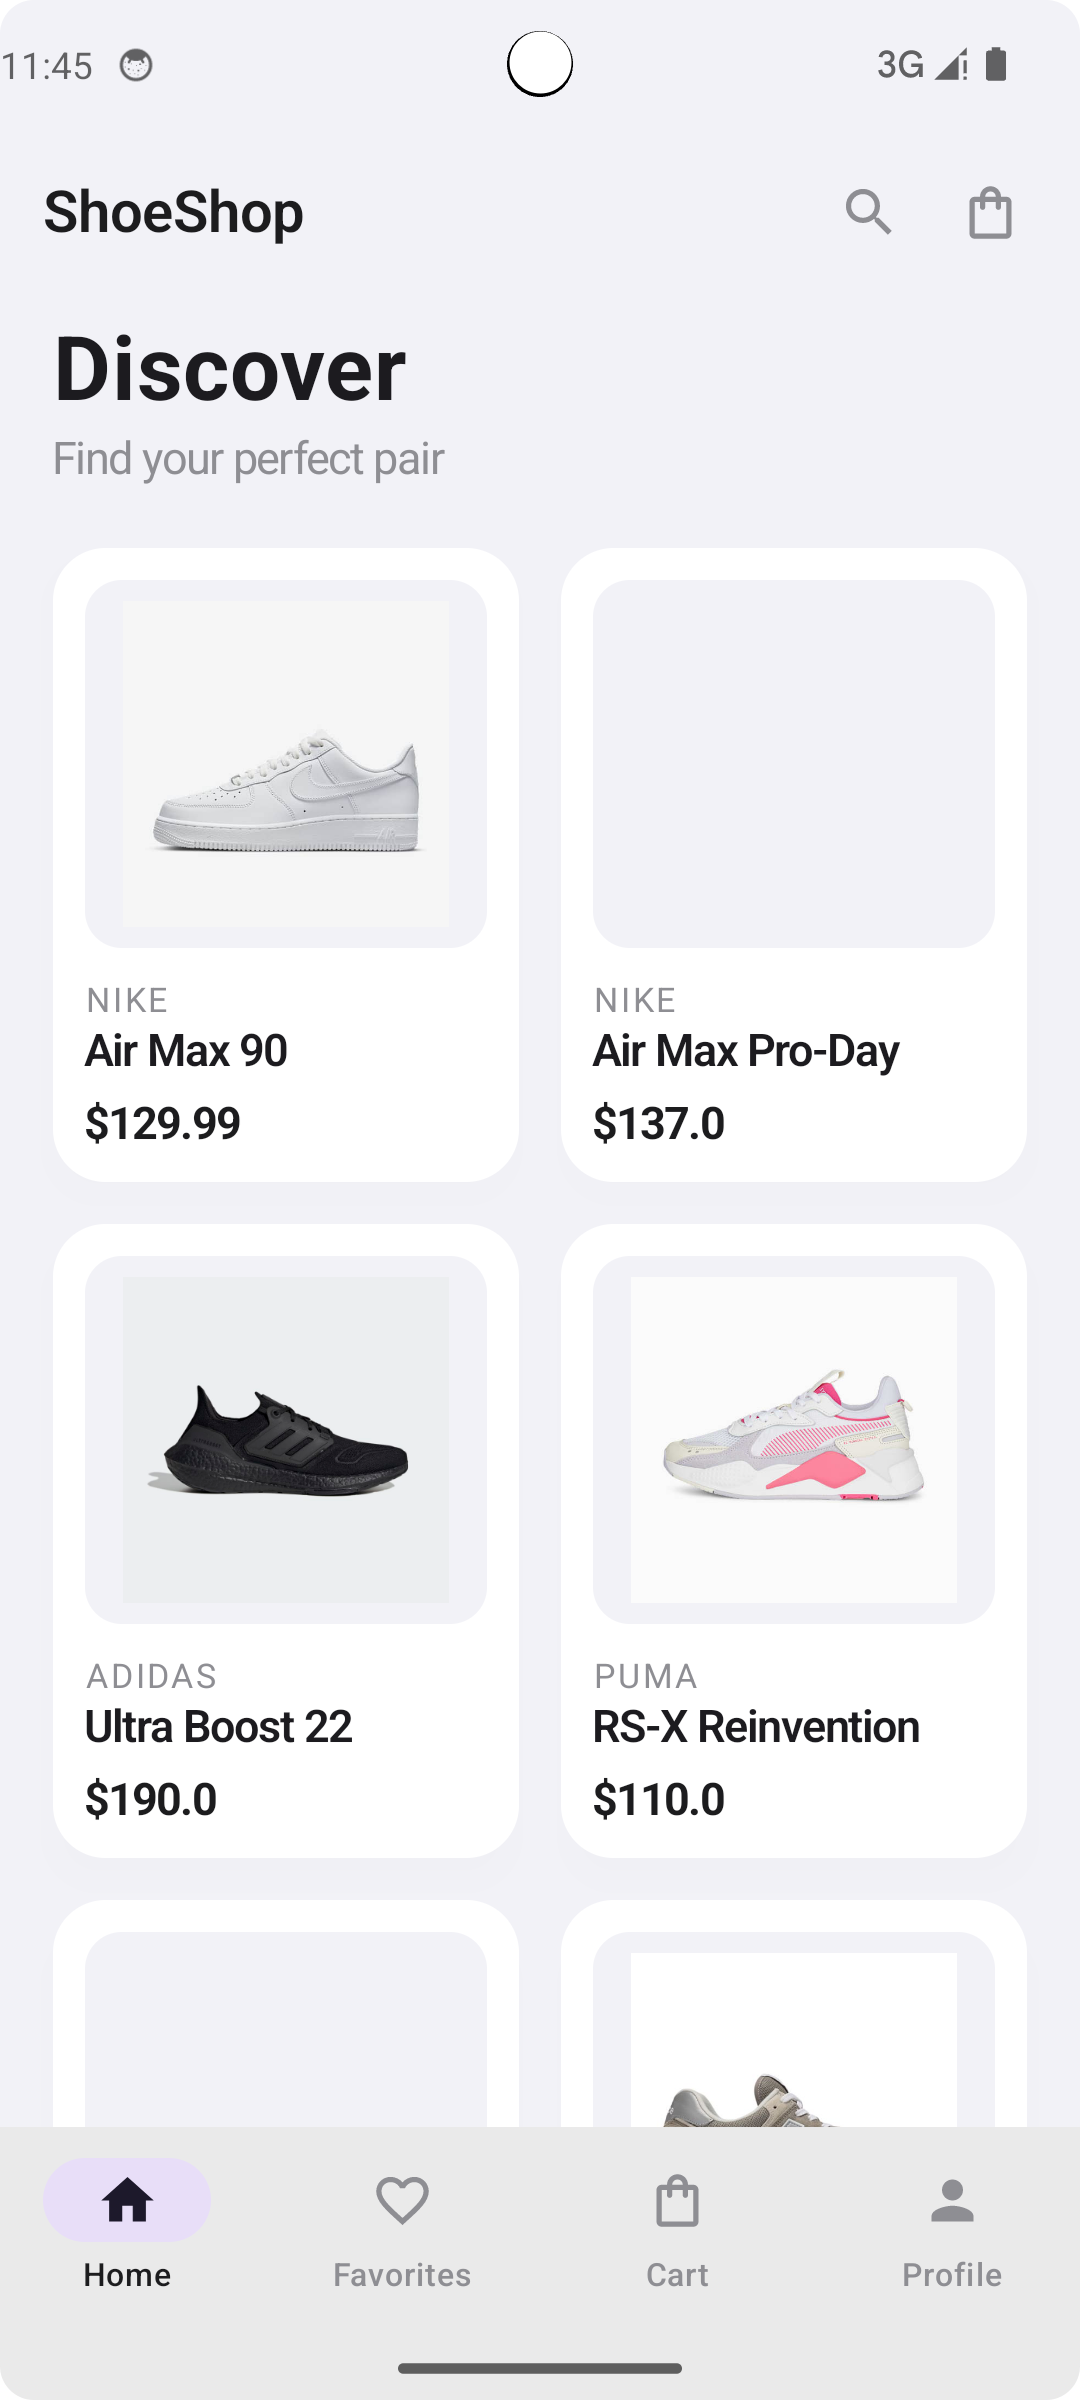
\includegraphics[width=0.4\textwidth]{Screenshots/Screenshot_20260504_234552.png}
\caption{Product catalog with M3 TopAppBar and NavigationBar}
\end{figure}

\subsection{Detail Screen}
\begin{figure}[H]
\centering
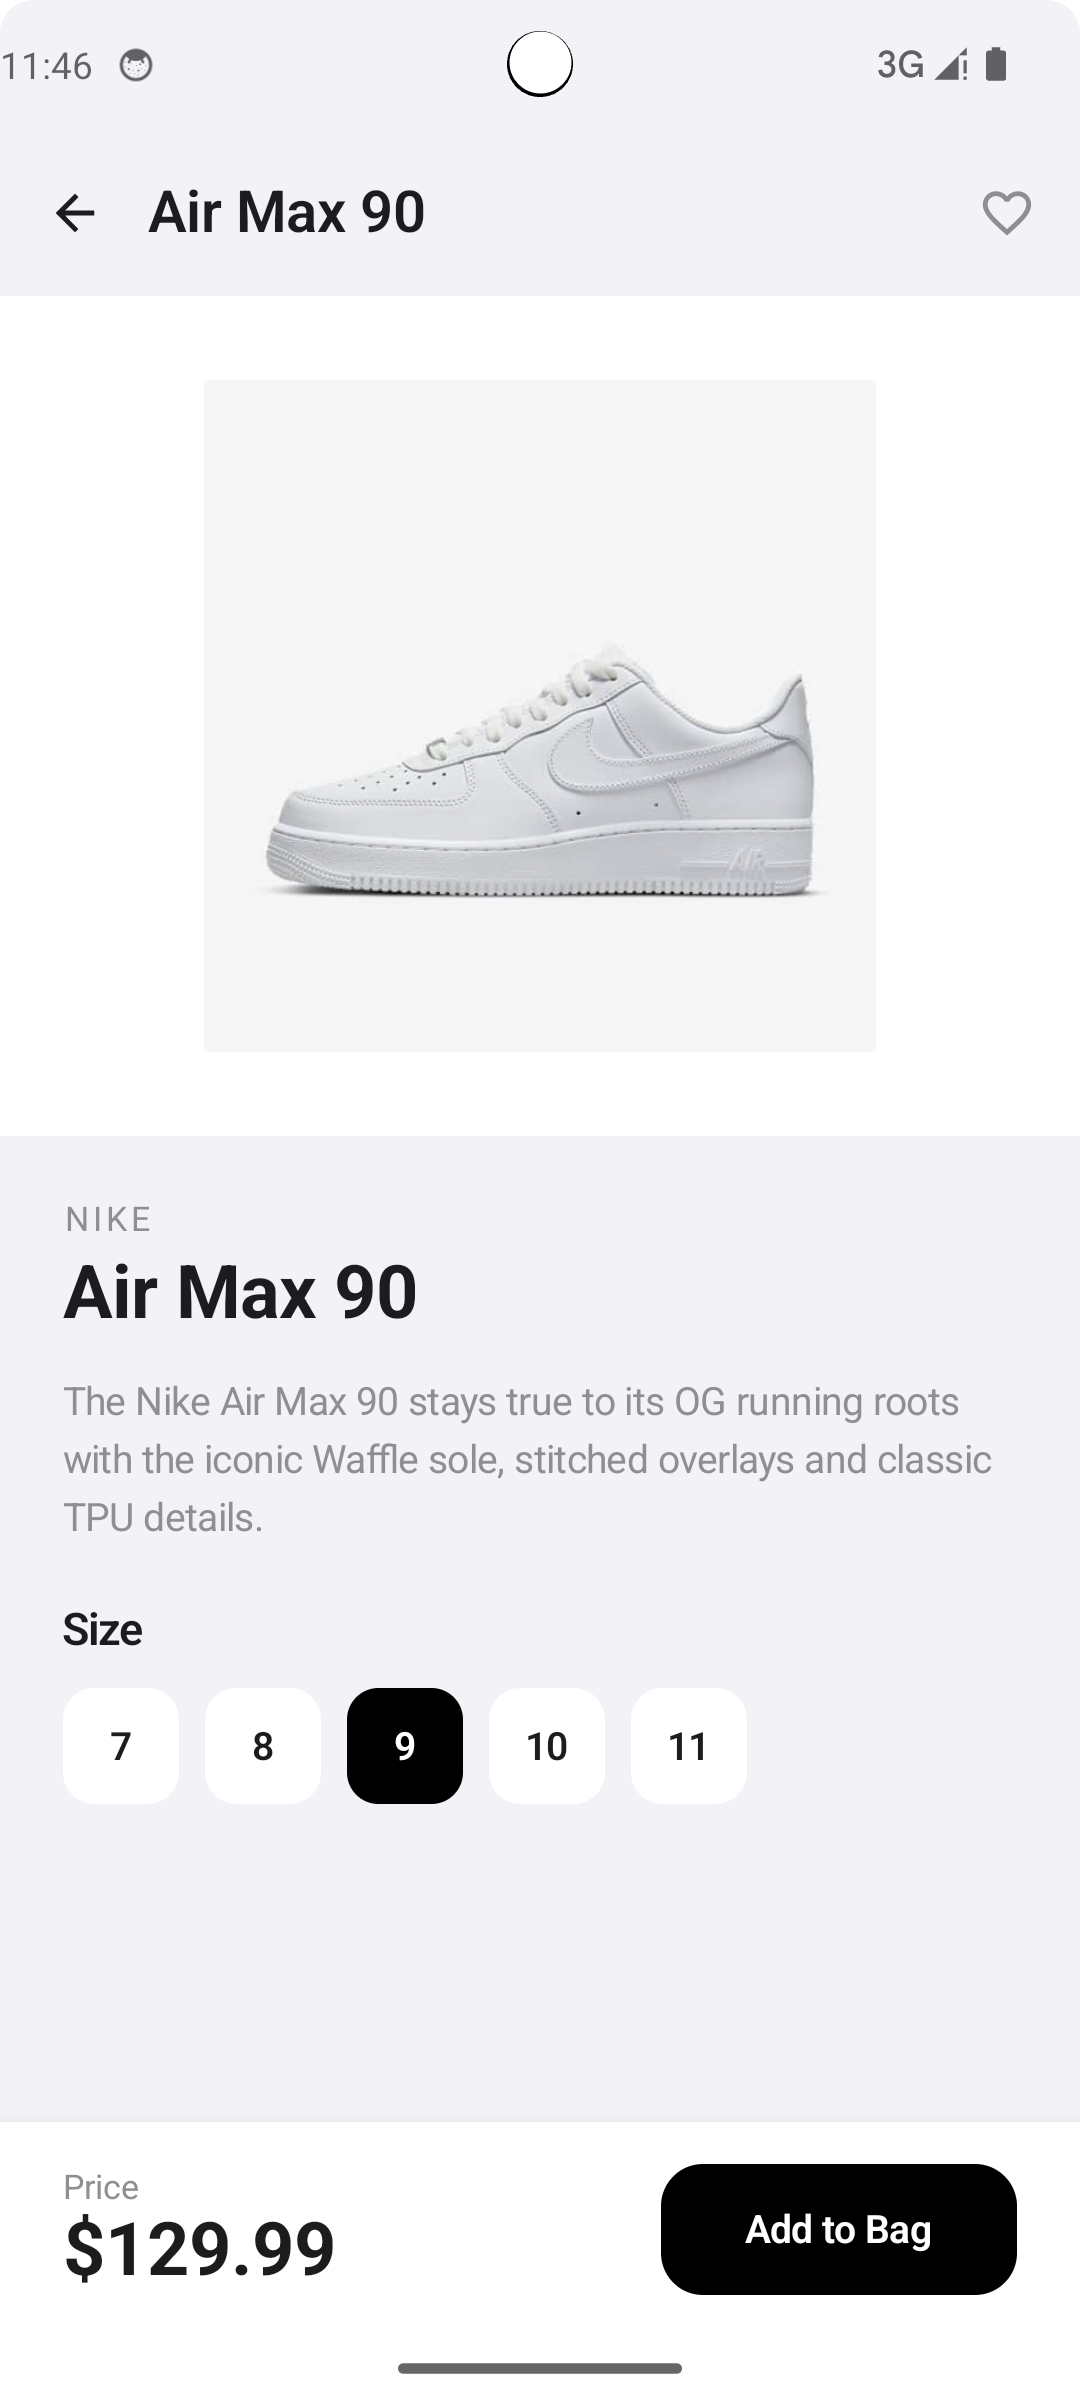
\includegraphics[width=0.4\textwidth]{Screenshots/Screenshot_20260504_234633.png}
\caption{Product detail with Scaffold, TopAppBar, and Add to Bag}
\end{figure}

\subsection{Shopping Cart}
\begin{figure}[H]
\centering
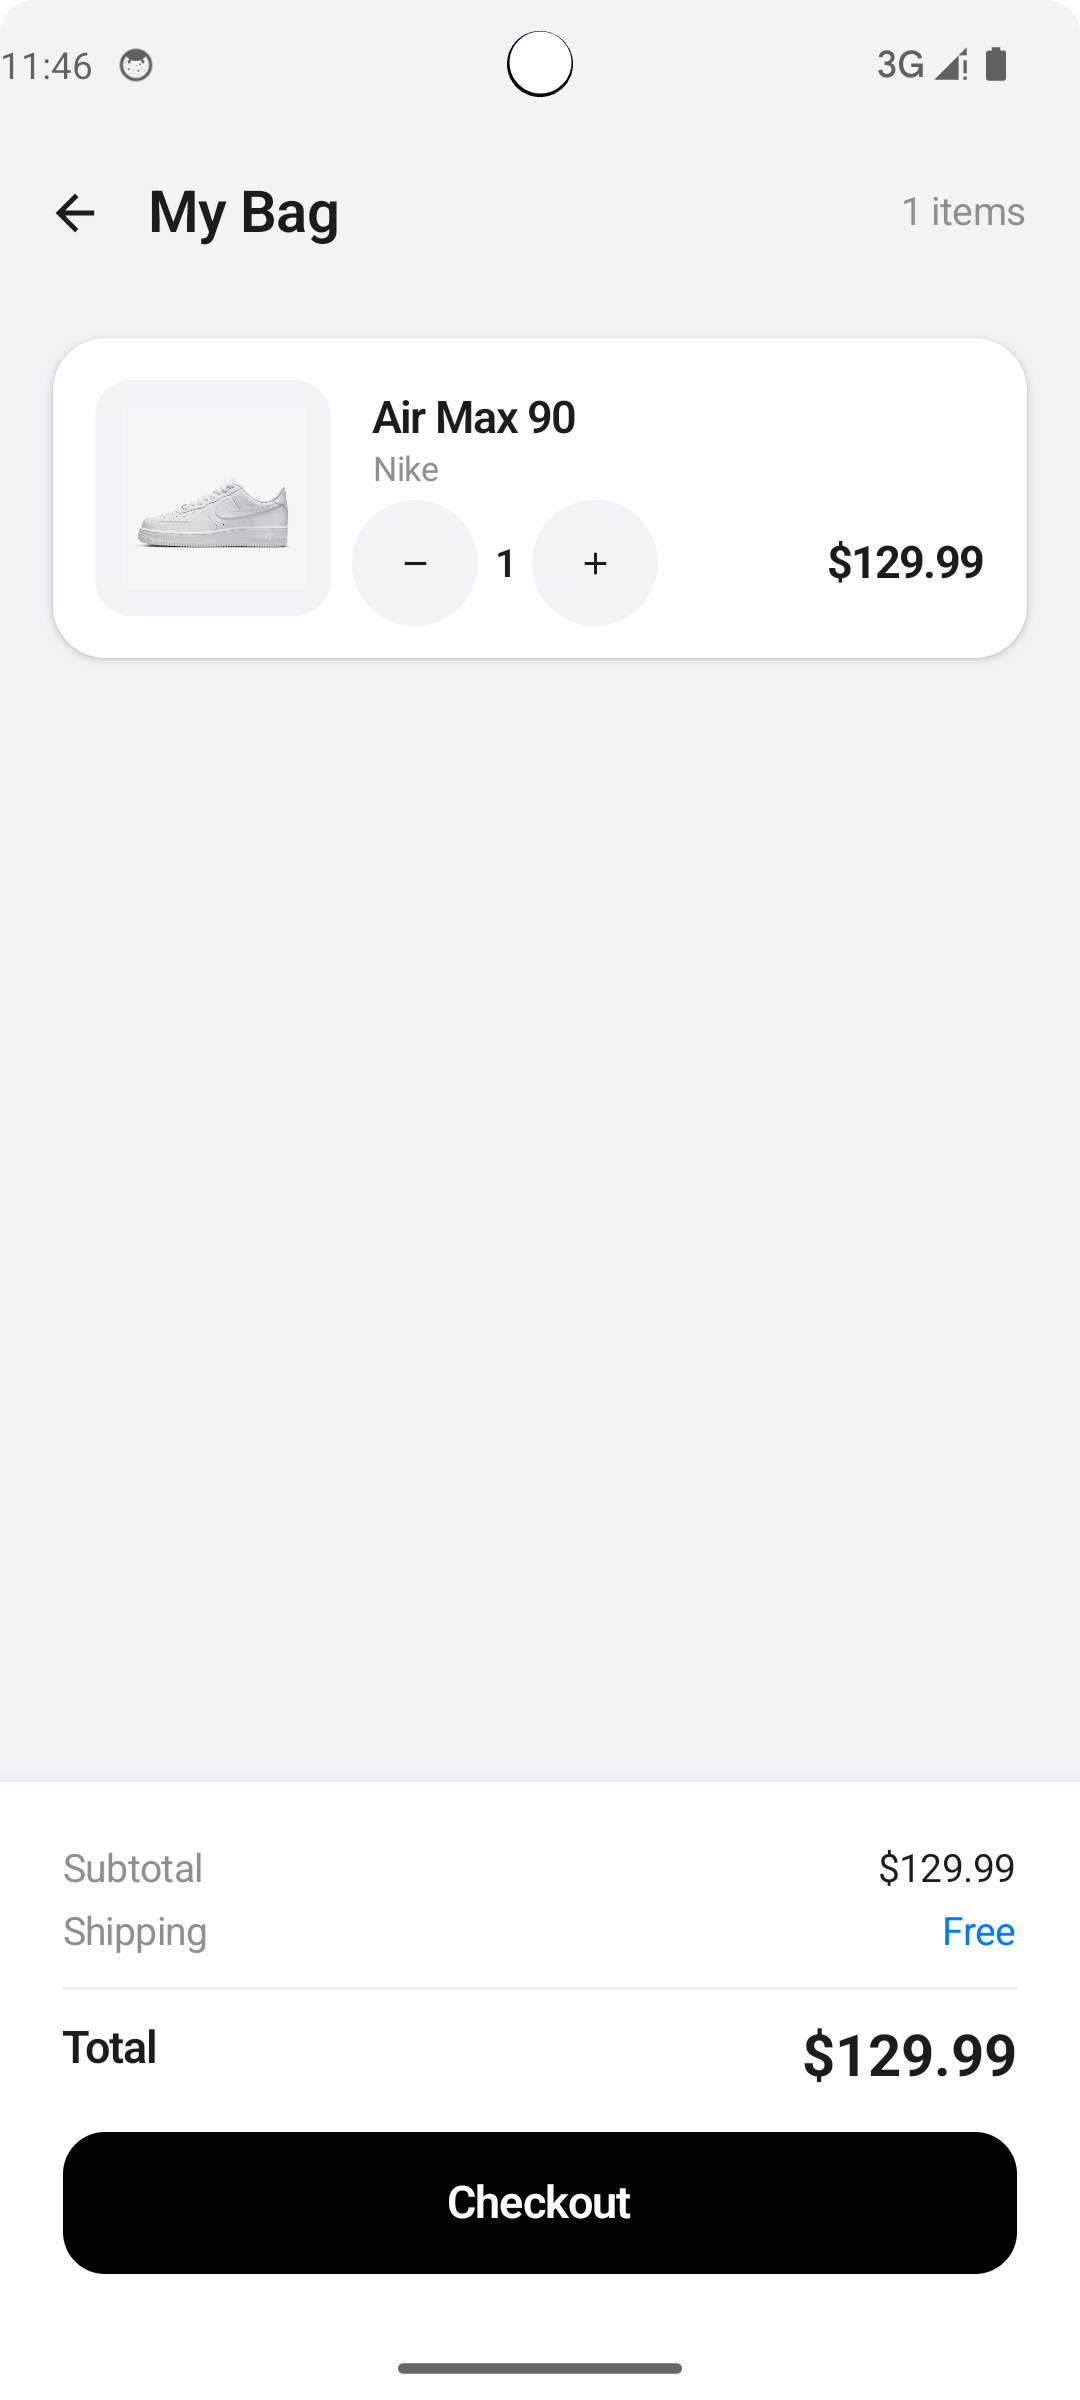
\includegraphics[width=0.4\textwidth]{Screenshots/Screenshot_20260504_234653.png}
\caption{Shopping bag with items and total calculation}
\end{figure}

\subsection{Cart with Multiple Items}
\begin{figure}[H]
\centering
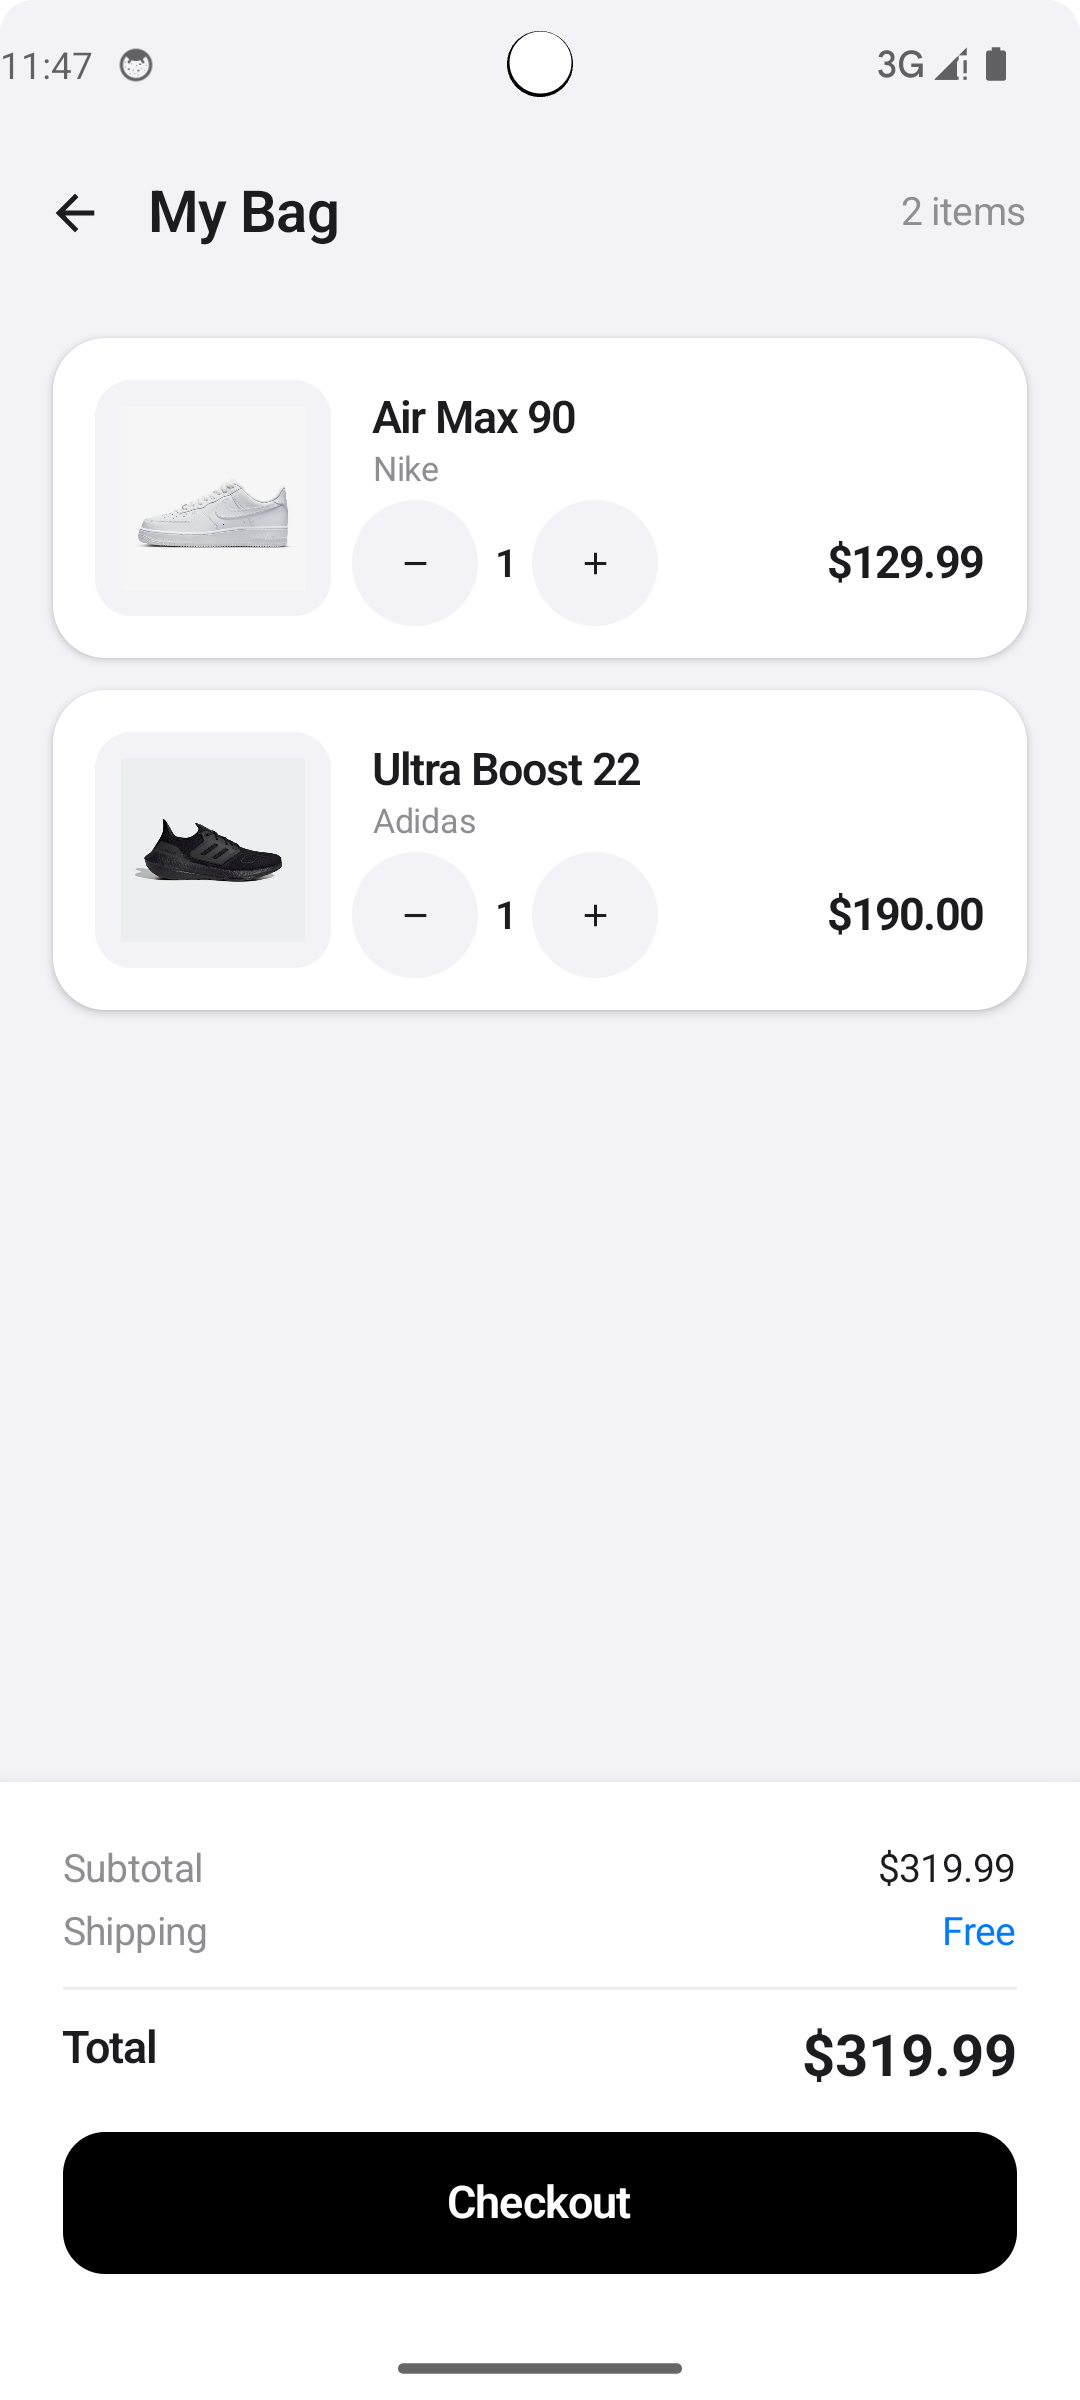
\includegraphics[width=0.4\textwidth]{Screenshots/Screenshot_20260504_234715.png}
\caption{Shopping bag with multiple items and quantity adjustment}
\end{figure}

\end{document}
